% !Mode:: "TeX:UTF-8"
\chapter{多线程}
\label{chap:java_thread}

上一章,不建议捕获Error类型的异常,对于单线程应用也没有实际意义。
但多线程的情况下,你不仅可以捕获,而且还能挽救业务。这是为什么呢?
现在,我们就带着这个问题,开始学习多线程的知识。
\vspace{1cm}

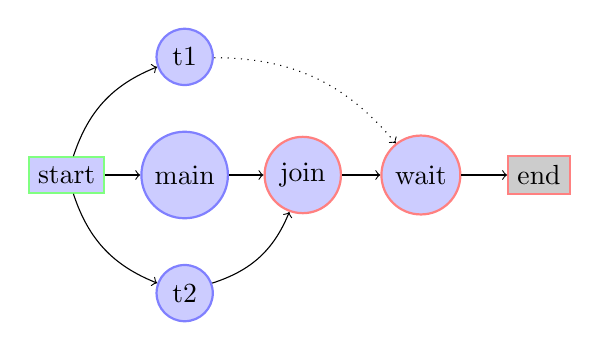
\begin{tikzpicture}[bend angle=25, node distance=1.5cm]
\tikzstyle{start}=[rectangle,draw=green!50,fill=blue!20,thick]
\tikzstyle{end}=[rectangle,draw=red!50,fill=black!20,thick]
\tikzstyle{run}=[circle,draw=blue!50,fill=blue!20,thick]
\tikzstyle{main}=[circle,draw=red!50,fill=blue!20,thick]
\node[run](t1){t1};
\node[run](t2)[below of=t1]  {main};
\node[run](t3)[below of=t2] {t2};

\node[main] (join) [right of=t2] {join}
	edge [<-]             (t2)
	edge [<-, bend left]  (t3);

\node[main](wait)[right of=join] {wait}
  edge [<-, bend right, dotted] (t1)
	edge [<-] (join);

\node[end](leave wait)[right of=wait] {end}
	edge [<-] (wait);

\node[start] (enter t2) [left of=t2]  {start}
	edge [->]            (t2)
	edge [->, bend left]  (t1)
	edge [->,bend right] (t3);

\end{tikzpicture}
\vspace{0.6cm}

上图,是一个多线程示意,包含3个线程。其中,中间那条执行线,称之为主线程。
上下执行线是2个单独的线程。多个线程一起工作,就需要一种互相协助的方法。
使用join可以使主线程等待t2执行完毕,再继续往后执行;
使用wait可以主线程等待t1执行完毕的通知,再继续往后执行。
线程在执行过程中,还可以sleep一段时间。\footnote{睡眠时间长度不保证精确。}

线程可分为:主线程、工作线程。其中,主线程负责UI的交互和刷新。
程序长时间等待不响应,就是你主线程卡住了。
所以,要避免在主线程消耗CPU,应该创建一个工作线程处理下载任务、读写大文件等。
再创建一个线程很简单,掌握\emph{同步}和\emph{异步}的用法才是本章的重点。

\section{创建线程}
通常,执行一个命令行程序,输出结果就退出了。譬如,\emph{dir}打印当前文件列表就结束了,
而启动\emph{python}就会进入交互模式,直到你显式请求退出。

\vspace{0.6cm}
\begin{figure}[!htb]
\begin{center}
\begin{tikzpicture}[bend angle=-25, shorten >=1pt,node distance=2.5cm,auto]
\node[startstop] (start) {start};
\node[runnable] (fork) [right of=start] {fork};
\node[process] (main) [right of=fork] {main};
\node[runnable] (t1) [above right of=fork] {run};
\node[startstop] (stop) [right of=main] {stop};
\path[->]
(start) edge node {执行} (fork)
(fork) edge [bend right] node {启动} (t1)
(t1) edge [bend right] node {退出} (stop)
(fork) edge node {主线程} (main)
(main) edge node {退出} (stop)
(t1) edge [loop above] node {耗时/异步} ();
\end{tikzpicture}
\end{center}
\caption{主线程和工作线程}
\end{figure}
\vspace{0.3cm}

主线程启动业务线程之后,就开始了各自的生命周期。
即使主线程先退出main函数,也还会等子线程结束才算程序退出。
这是线程的第一种用法:创建并启动线程,相互独立运行。

\begin{lstlisting}
	Section_5_1: main exit!
	Section_5_1: end of main!
	Section_5_1: thread exit!
\end{lstlisting}

在主线程退出之后,就不能再响应用户的输入和点击。英文单词\emph{Thread}是
线程的类名,创建对象是\lstinline{t=new Thread()},启动它用\emph{t.start()}。
很显然这样一个线程什么都做不了。由面向对象知识,可通过\lstinline{@Override}
run方法重写线程代码。

\begin{lstlisting}[language=Java,mathescape]
		// 1. 匿名方式继承Thread重写run方法
		Thread t1 = new Thread() {
			@Override
			public void run() {
					// do something
			}
		}
		// 2. 匿名方式实现Runnable
		Thread t2 = new Thread(new Runnable() {
			@Override
			public void run() {
					// do something
			}
		}
		// 3. lambda方式实现Runnable
		Thread t3 = new Thread(()-> {
				// do something
		}
\end{lstlisting}

上述三种方式,t1和t2很相似但不同,而t3最简单。在JDK8之前,最常使用第2种方式创建线程。

\section{线程协作}
在本节内容开始之前,有必要先认识一下Java是如何执行的。
首先把Java文件编译成class或者jar,再启动JVM把它们加载到内存,找到主类从它的main函数
开始执行的。进程(Process)是操作系统分配资源(内存、CPU)的最小单位,
所有的线程都运行在该进程空间中。你创建的对象都被放在堆内存中,所有的线程都可以访问它。

实际上,内存被划分为若干个区域:堆区、栈区和方法区等。其中堆区是所有线程共享的,
也是所有对象的存放地。而栈主要是用来执行代码的,在函数调用过程中参数传入弹出,
都是在这个栈里面。很显然,栈空间就是存放临时数据的,用于准备参数给函数调用。
使用完之后,就会规划栈区空间。所以栈是一个来回复用的地方,而我们的局部变量和参数一样,
也是在栈区,函数返回之后,局部变量也就出栈了。但是那个内存地址的数据,可能没有擦除。
这就要求我们,定义的局部变量一定要初始化!

栈的这种特性,决定了它不需要分配太多的内存。但如果递归调用或者函数调用层次太深,
必将出现栈溢出!每次函数调用,都要把参数和函数的局部变量入栈,生成一个栈帧。
所以,在使用递归的时候,务必要注意不要太深(大约1W次)。

\begin{figure}[!htb]
\centerline{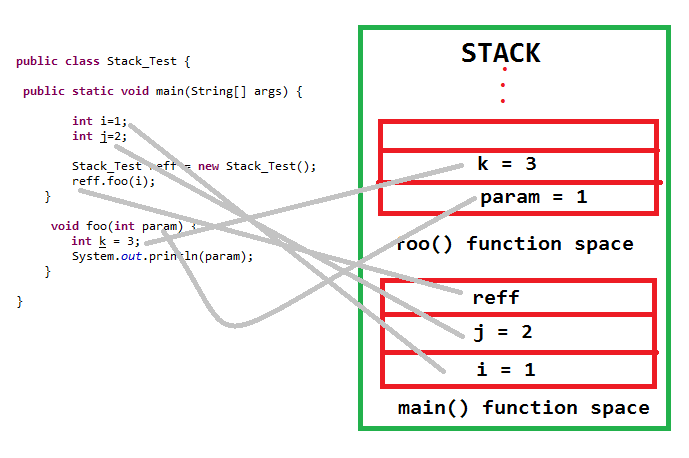
\includegraphics[width=.4\figwidth]{images/stack_memory_space.png}}
\label{fig:part1_thread_stack}
\caption{线程栈帧}
\end{figure}

每个线程都有自己的栈空间,不是共享的。
在Java中,创建的对象都在堆空间里,而栈空间基本都是对象的引用。
上图中,栈中的name指向外部的字符串对象。每个线程都有各自的栈空间,互相独立使用。

\subsection{wait和notify}
等待(wait)和通知(notify),是常见的多线程同步方法,比起轮询要好。
尤其是,有好几个线程的时候,最好使用这种机制(或者同步块)。
从字面意思理解,也很容易使用。当缺少继续运行条件的时候,就让当前线程
进入等待(wait)状态,而其它线程致使条件成立之后notify它。
假设,现在有T1、T2、T3、T4四个线程,其中T1、T2、T3都在等待条件C1,
只有T4处理完才会发布C1条件。
\vspace{0.2cm}

\noindent
1. 锁对象,任何Java对象或类,都可以作为锁。
\begin{lstlisting}[language=Java]
	void print(String info) {
		System.out.println(info);
	}

	private Object C1 = new Object();

	void doLocked(Object lock) {
		try {
				lock.wait();
		} catch (InterruptedException e) {
				e.printStackTrace();
		}
	}
\end{lstlisting}
\noindent
\begin{center}
\begin{minipage}{\textwidth}
\begin{parcolumns}{2}
\colchunk{
2. 创建多个线程,等待C1的唤醒。
\begin{lstlisting}[language=Java]
	Thread T1 = new Thread(() -> {
		print("T1: enter");
		synchronized (C1) {
				print("T1: process");
				doLocked(C1);
		}
		print("T1: done");
	});
	Thread T2 = new Thread(() -> {
		print("T2: enter");
		synchronized (C1) {
				print("T2: process");
				doLocked(C1);
		}
		print("T2: done");
	});
\end{lstlisting}}
\colchunk{
\begin{lstlisting}[language=Java]
	Thread T3 = new Thread(() -> {
		print("T3: enter");
		synchronized (C1) {
				print("T3: process");
				doLocked(C1);
		}
		print("T3: done");
	});
	Thread T4 = new Thread(() -> {
		print("T4: enter");
		synchronized (C1) {
				sleep(3000);
				C1.notify();
		}
		print("T4 exit!");
	});
\end{lstlisting}}
\colplacechunks
\end{parcolumns}\end{minipage}\end{center}
\noindent
3. 启动所有线程,T1、T2、T3虽然会先执行,但很快都会处于wait状态。
\begin{lstlisting}[language=Java]
	T1.start();
	T2.start();
	T3.start();
	T4.start();
\end{lstlisting}

\noindent
上述例子,使用C1作为锁,也可以使用\lstinline{C1=类.class},
譬如\lstinline{C1=Object.class}。使用notify会随机唤醒一个线程,
由于选择是任意性的,在设计JAVA程序时,不要依赖于这一点。
notifyAll可唤醒所有等待C1的线程并允许它们获得对象锁,但并不是同时获得执行权。
synchronied块中的代码,只能有一个线程运行。
所以,唤醒一个线程就是允许这个线程获得C1对象锁并继续往下运行。 
notifyAll对每个wait对象顺序调用一次notify,逐个唤醒线程。

值得注意的是,执行wait之前必须先获得对象锁,必须先进入\lstinline{synchronized}
代码块。调用wait之后,就会让出C1给其它线程抢占。但是上述例子,T1即使让出C1锁,线程T2和T3
已经提前进入等待队列,不会查询C1锁的状态,只有使用notify、notifyAll才能
唤醒它们。

使用\lstinline{synchronized}的时候,代码块要尽量小。
它不仅可以包含代码块,还可以放在函数名前面保护整个函数,这就是比较大的同步块。

\begin{lstlisting}[language=Java]
	synchronized void doLocked(String info) {
		try {
				print(info);
				wait();
		} catch (InterruptedException e) {
				e.printStackTrace();
		}
	}

	Thread T1 = new Thread(() -> {
		print("T1: enter");
		doLocked("T1: process");
		print("T1: done");
	});

	Thread T4 = new Thread(() -> {
		synchronized (this) {
				sleep(3000);
				notify(); // this.notify();
		}
		print("T4 exit!");
	});
\end{lstlisting}
从JDK5开始,新增的java.util.concurrent包提供了更多的同步机制,
譬如ReentrantLock、ReadWriteLock。
使用Lock不需要\lstinline{synchronized},但需要你主动释放锁。

\begin{lstlisting}[language=Java]
private Lock lock = new ReentrantLock();// 锁对象
....
lock.lock();// 得到锁
....
lock.unlock();// 释放锁  
\end{lstlisting}

\noindent
限于篇幅不再展开,通常使用\lstinline{synchronized}就可以解决所有同步问题。

\section{线程池}
创建线程后,并做一系列的初始化,肯定会消耗不少的时间。
尤其是网络读写和数据库初始化可能要十几秒才能完成。
这对时间有严苛要求的任务,是无法接受的。
所以,需要一种复用线程的方案,随时都能有一个准备的线程。只要把Task递给线程池,
它就会线程池中,挑选一个空闲的执行任务,除非线程池是空的才会新建工作线程。
并且,新建的线程用完之后,也会放到线程池里面。

对于刚接触编程的同学,实现一套线程池代码难度很高。在java.uitl.concurrent
包中,JDK提供了ThreadPool实现,其中,ThreadPoolExecutor是线程池的核心类,

\begin{figure}[!htb]
\centerline{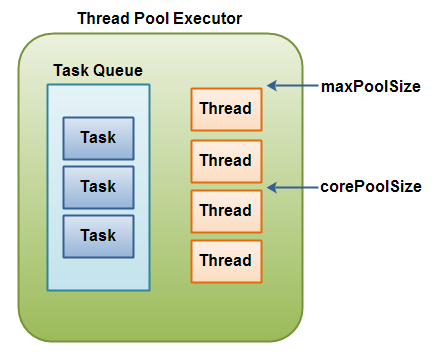
\includegraphics[width=.25\figwidth]{images/thread-pool-executor.png}}
\label{fig:part1_thread_pool}
\caption{线程池}
\end{figure}

\noindent
如上\figref{fig:part1_thread_pool},线程池有3个核心概念:corePoolSize、
maxPoolSize和TaskQueue。
其中,corePoolSize代表初始准备的线程数,也是最少的线程数;
maxPoolSize代表最多可以保留多少个线程;TaskQueue很显然是任务数超出maxPoolSize
的时候,Task就要入队等待。

\begin{lstlisting}[language=Java]
pool.schedule(() -> print("Task1 delay 3 seconds"), 3, TimeUnit.SECONDS);
pool.schedule(() -> print("Task2 delay 2 seconds"), 2, TimeUnit.SECONDS);
pool.schedule(() -> print("Task3 delay 1 seconds"), 1, TimeUnit.SECONDS);
pool.schedule(() -> print("Task4 delay 4 seconds"), 4, TimeUnit.SECONDS);
pool.schedule(() -> print("Task5 delay 5 seconds"), 5, TimeUnit.SECONDS);
pool.schedule(() -> print("Task6 delay 6 seconds"), 6, TimeUnit.SECONDS);
\end{lstlisting}

\noindent
在主线程退出main函数之后,线程池并不会退出,除非你主动\lstinline{pool.shutdown();}
才能看到\lstinline{Process finished with exit code 0}。

\section{总结}
限于本书篇幅,不能覆盖所有多线程的知识,通过本章的学习至少可以达到管中窥豹的效果。
线程池在高性能、数据处理和Web开发用的比较多,初学Java多线程,
掌握Thread和Synchronized就可以了。